\documentclass{sigchi}

% Use this command to override the default ACM copyright statement (e.g. for preprints).
% Consult the conference website for the camera-ready copyright statement.


%% EXAMPLE BEGIN -- HOW TO OVERRIDE THE DEFAULT COPYRIGHT STRIP -- (July 22, 2013 - Paul Baumann)
% \toappear{Permission to make digital or hard copies of all or part of this work for personal or classroom use is 	granted without fee provided that copies are not made or distributed for profit or commercial advantage and that copies bear this notice and the full citation on the first page. Copyrights for components of this work owned by others than ACM must be honored. Abstracting with credit is permitted. To copy otherwise, or republish, to post on servers or to redistribute to lists, requires prior specific permission and/or a fee. Request permissions from permissions@acm.org. \\
% {\emph{CHI'14}}, April 26--May 1, 2014, Toronto, Canada. \\
% Copyright \copyright~2014 ACM ISBN/14/04...\$15.00. \\
% DOI string from ACM form confirmation}
%% EXAMPLE END -- HOW TO OVERRIDE THE DEFAULT COPYRIGHT STRIP -- (July 22, 2013 - Paul Baumann)


% Arabic page numbers for submission. 
% Remove this line to eliminate page numbers for the camera ready copy
% \pagenumbering{arabic}


% Load basic packages
\usepackage{balance}  % to better equalize the last page
\usepackage{amssymb}  % mathematical symbols
\usepackage{graphics} % for EPS, load graphicx instead
\usepackage{pgfplots} % Bar charts
\usepackage{times}    % comment if you want LaTeX's default font
\usepackage{url}      % llt: nicely formatted URLs
\usepackage[utf8]{inputenc}
\usepackage{soul}
\sethlcolor{black}

\usepackage{tikz}
\usepackage{subcaption}

% llt: Define a global style for URLs, rather that the default one
\makeatletter
\def\url@leostyle{%
  \@ifundefined{selectfont}{\def\UrlFont{\sf}}{\def\UrlFont{\small\bf\ttfamily}}}
\makeatother
\urlstyle{leo}


% To make various LaTeX processors do the right thing with page size.
\def\pprw{8.5in}
\def\pprh{11in}
\special{papersize=\pprw,\pprh}
\setlength{\paperwidth}{\pprw}
\setlength{\paperheight}{\pprh}
\setlength{\pdfpagewidth}{\pprw}
\setlength{\pdfpageheight}{\pprh}

% Make sure hyperref comes last of your loaded packages, 
% to give it a fighting chance of not being over-written, 
% since its job is to redefine many LaTeX commands.
\usepackage[pdftex]{hyperref}
\hypersetup{
pdftitle={SIGCHI Conference Proceedings Format},
pdfauthor={LaTeX},
pdfkeywords={SIGCHI, proceedings, archival format},
bookmarksnumbered,
pdfstartview={FitH},
colorlinks,
citecolor=black,
filecolor=black,
linkcolor=black,
urlcolor=black,
breaklinks=true,
}

% create a shortcut to typeset table headings
\newcommand\tabhead[1]{\small\textbf{#1}}

\newcommand{\nm}{\normalsize}

% End of preamble. Here it comes the document.
\begin{document}

\title{Towards Touch-Based Medical Image Diagnosis Annotation}

\numberofauthors{4}
\author{
\alignauthor { Francisco M. Calisto}\\
\affaddr{ Institute for Systems and Robotics (ISR/IST), LARSyS, Instituto Superior T\'{e}cnico, Univ Lisboa}\\
\email{\nm francisco.calisto@tecnico.ulisboa.pt}\\
%\affaddr{Optional phone number}
\alignauthor { Alfredo Ferreira}\\
\affaddr{INESC-ID, Instituto Superior Técnico, Universidade de Lisboa}\\
\email{\nm alfredo.ferreira@tecnico.ulisboa.pt }\\
%\affaddr{Optional phone number}    
\alignauthor { Daniel Gonçalves}\\
\affaddr{INESC-ID, Instituto Superior Técnico, Universidade de Lisboa}\\
\email{\nm daniel.j.goncalves@tecnico.ulisboa.pt}\\
%\affaddr{Optional phone number}
\alignauthor { Jacinto C. Nascimento}\\
\affaddr{ Institute for Systems and Robotics (ISR/IST), LARSyS, Instituto Superior T\'{e}cnico, Univ Lisboa}\\
\email{\nm jacinto.nascimento@tecnico.ulisboa.pt }\\
%\affaddr{Optional phone number}    
}

\maketitle

\begin{figure}[h]
\centering
\includegraphics[width=1.0\columnwidth]{header_1.jpg}
\caption{Radiologist interacting with traditional environment.}
\label{fig:Fig1}
\end{figure}

\begin{figure}[h]
\centering
\includegraphics[width=1.0\columnwidth]{header_2.jpg}
\caption{Touch environment interaction.}
\label{fig:Fig2}
\end{figure}

\begin{abstract}

A fundamental step in medical diagnosis for patient follow-up relies on the ability of radiologists performing reliable diagnosis from acquired images. Basically, the diagnosis strongly depends on the visual inspection over the shape of the lesions, and somehow register its evolution through time. In existing clinical setups, a large number of images are currently acquired and should be individually inspected. As datasets increase in size, such visual evaluation becomes harder. For this reason it is crucial to introduce easy-to-use interfaces that help the radiologists not only to perform a reliable visual inspection but more importantly, allow the efficient delineation of the lesions. In this paper, we will present a study on integrating the above interfaces in a real-world scenario. More specifically, we will explore the radiologist's receptivity to the current touch environment solution. The advantages of touch are threefold: (i) the time performance is superior regarding the traditional use, (ii) it has more intuitive control and, (iii) for less time, the user interface delivers more information per action, concerning annotations. We concluded, from our studies that the path towards touch-based on medical image diagnosis annotation includes overcoming the current refusal to use these systems by radiologists, which resist change.  Also, a solution to the finger occlusion must be devised.

\end{abstract}

\keywords{
	Touch-Based; Medical Image Diagnosis; Medical Visualization; Interaction Design; Human-Computer Interaction
}

\category{H.5.2.}{Information Interfaces and Presentation (e.g. HCI)}{User Interfaces}

\section{Introduction}

Medical imaging diagnosis is a topic of great interest, that has been the subject of intensive research in the field of medicine, and more specifically in Radiology~\cite{doi2007computer, seibel2005medical, doi2005current}. However, current tools do not fully support annotation collection. These annotations and their relationships are crucial for a proper diagnosis. Namely, to have the morphological time evolution of potential lesions that may be present in some organs.

In this paper, we present a performance and experience analysis conducting a study of touch and traditional environments (Figures \ref{fig:Fig1} and \ref{fig:Fig2}) that are aligned to the previous mentioned goals. Both environments are  comfortable to interact with and fast enough to solve the annotation tasks. For each environment, the same simple image feature (e.g. delete/correct annotation) is considered.

The performance differences of traditional and touch input devices have been studied~\cite{watson2013deconstructing} in terms of speed and accuracy for a variety of clinical and medical interactive tasks. This includes features such as Regions of Interest (ROI) annotations and length measurements, among others. Although, user experience while inserting annotations is important when evaluating the input devices, there is still a lack of research examining how the experience compromises the interactive surfaces based on the input type. To tackle this, our main goals focus primarily on cognition and time-performance. The experience is also considered as a means to validate the sensation, affect and value of  interaction.

Indeed, while user experience analysis and evaluation has been applied to clinical systems~\cite{crisan2013optimization},  time-measure and error scales are still missing. Moreover, a touch interactive surface application can improve medical and clinical competences, since it is able reduce the running time figures to complete common tasks in the diagnosis loop.

Considering the most basic elements of interaction development for medical imaging annotations, we use the following annotation tasks: (i) \textit{ROI}, (ii) \textit{enabling}, (iii) \textit{disabling}, (iv) \textit{activate}, (v) \textit{deactivate}, (vi) \textit{clear all} and (vii) \textit{change image} in a casual medical and clinical application. We conducted an experimental study comprising five participants and two distinct environments: traditional and touch based environments.

Experimental evaluation demonstrates that, although the radiologists prefer to maintain their current workflow based on traditional environments, using a touch interface they are able to provide more annotations. Such increment contributes for the efficiency at delineating structures in medical images. We concluded that, for less time radiologists delivered more information per action on the user interface. Also, we observed that touch environments have more intuitive controls and provides a more pleasant interaction.

\section{Related Work}

In this section we describe the most relevant techniques used for both touch and traditional environments. 
%It focus, primarily on the performance metrics, to find an increase in performance of tasks, requiring less time and producing more and better results. 
An early work~\cite{shanis2003comparison} showed that touch environments beat traditional ones when performing target selection, which has significant impact in terms of speed, but a decrease when performing shape matching~\cite{forlines2007direct}. On the other hand, some other works~\cite{tan2002kinesthetic, wallace1972spatial, nacher2016kindergarten} found an increase in the performance of tasks that require recall and spatial memory when using touch devices. A quality of experience in touch tasks showed to be more efficient than the traditional ones when doing target acquisition tasks of shape docking and moving targets tasks.

A comparison of user performance with three relative devices on a desktop display and two  orientations, using a small vertical display, is presented in~\cite{meyer1994device}. Here, they found that the touch screen environment resulted in the worst performance  when compared to traditional environments. However, in~\cite{accot1997beyond} they highlight that for steering tasks users are about twice as fast on the touch environments.

Other authors~\cite{benko2006precise, esenther2006fluid} investigated the use of additional fingers to mode the mapping between touches and control point on displays. In this manner, a radiologist is able to switch to a slower and more accurate mapping, when detailed control is needed and can default back to direct single-finger input when working with larger targets.

Albinsson and Zhai~\cite{albinsson2003high} compared a collection of input techniques designed to improve the accuracy of bare hand interaction with a touch environment. 
They found that performance and preferential interaction lines depend on the target size, leading to different performance rankings. Also, they conclude that system should provide to the radiologists a variety of selection tools, so that the radiologist can choose the most appropriate tool for the task.

In the seminal work of Card, English and Burr's~\cite{card1978evaluation} on the quantitative comparison of pointing devices, it is shown that indirect traditional input environment compared  favorably to direct stylus input. While there are important differences between stylus and touch input environment, one would expect that these results might generalize to single-finger pointing.

Sears and Shneiderman~\cite{sears1991high} compared traditional and touch screen inputs in a single task, investigating the differences of the above input environments for the tasks on a variety of displays. It becomes apparent that system developers need to consider the proportion of the input that their system requires when choosing between touch and traditional input environments~\cite{forlines2007direct}. While a touch input environment modality may not lead to greater performance in terms of speed and accuracy for the single tasks, other considerations, such as fatigue, spatial memory, and awareness of other’s actions, might convince a system developer to choose single-interactions input over traditional input environments.

Among the earliest work in the Human Computer Interaction field is the study of Buxton and Myers~\cite{kabbash1994two}, which clearly articulated the benefits of input on radiologist interface tasks. This body of research has typically investigated interaction with traditional environments or in virtual reality~\cite{sousa2017vrrrroom} environments, but not in tabletop settings. Balakrishnan and Hinckley~\cite{balakrishnan1999role} investigated the value of proprioception in asymmetric bi-manual tasks. They found that radiologists benefit from working in a single absolute reference frame when completing bi-manual tasks when visual feedback is absent.
%, but that the benefit diminishes when visual feedback is provided.

Latulipe et al.~\cite{latulipe2005bimanual, latulipe2006symspline} studied symmetric inputs performed with traditional environments. They found that for many tasks, symmetric inputs outperforms not only single interaction, but also asymmetric inputs in terms of performance and preference, and advocate the addition of a second interaction on traditional environment. Barnert~\cite{barnert2005comparison} describes an experiment in which participants performed better when using traditional environment than when using touch environment directly on a table while completing an asymmetric task. Because the task used in this study required pixel-accurate positioning, the author suggests that the superior performance of the traditional environment may be due to the relatively large size and low accuracy of one’s fingertips.

Other issues of interest are the interactive angle for the touch environments. Ahlstr\"{o}m and Lenman~\cite{ahlstrom1990fatigue} studied this behavior on their work investigating how the screen angel affects the user performance and fatigue. The fact that the standard monitor position used by traditional environments is not optimal, at least when using a touchscreen, is supported by these studies.

Another relevant aspect that deserves interest is the presence of bias.
This can be regarded as the consistent differences between the location that users want to touch, and where they actually touch
\cite{beringer1985underlying, beringer1989operator}. Concerning the biases  created by radiologists at various positions relative to the touch environments, the results in~\cite{hall1988factors} indicate that touch biases depend on viewing angle.

In summation, while the use of touch or traditional environments is not new in a medical and clinical settings, combining them for medical imaging diagnosis has not been studied. Much of the research focuses on the comparison between touch and traditional environments. 

Although, our approach does not address diagnosis, it is of crucial importance to observe the radiologist's behaviour on their typical environment and how they actually work. Moreover, we specifically work with health professionals in both traditional and touch environments interactions. The above environments are  purposely introduced to combine novel, yet familiar, touch gestures with immersive visualization.

In this paper we focus on time performance and human error reduction and adding more understanding about time performance relation between both aforementioned environments.

\section{Context}

In the attempt to meet the usual work conditions that radiologist's have,  we brought the most common interaction work space into the hospital meeting room. The experiments were conducted at the radiology services of Hospital \hl{Fernando Fonseca, Lisbon}. The radiologists are sitting on the most comfortable position in front of both traditional and touch environments. An experiment was designed by us to better understand performance between traditional and touch input environments. More specifically, we are interested in developing a deeper understanding of a radiologist's needs for motivation and satisfaction, when using touch environments and comparing conditions to better understand the obtained results through standard methods of time performance (e.g. number of interaction annotations and hit rate score).

\subsection{Procedure}

The experiment was carried out on two consecutive days. In each day, the  radiologists performed two repetitions, one for each environment, for a given task. The task consists the delineation of the same mass lesion (tumor) in three different frames. Each frame is a DICOM Magnetic Resonance Image (MRI) of the brain~\cite{mildenberger2002introduction} containing a mass lesion near the cortex. In the first two images, the lesion exhibits a similar shape since the view is almost the same. In the third image the view is different, where now the MRI has a frontal view of the brain (Figure \ref{fig:Fig6}), and the lesion exhibits a more irregular shape, being more difficult to be delineated.
 
For each environment, the radiologists participated in a one minute of training session with the researcher explaining the interface features that must be followed to perform the shape annotation. Then, the radiologist is asked to perform, as in training sessions, the same task on the three DICOM-MRI images and with no external researchers intervention. When the tasks for each image are successfully completed, the radiologist has to press the ``Next'' button, to be able to access the next image. If the researcher observed that the radiologist did not carry out the task in a given time, this is marked as incomplete task. All the user interactions are recorded in videos, we also recorded the heat maps 
and the coordinates. 

\section{Evaluation}

Performance and experience are addressed within-subjects design with both input environments devices. The traditional environment concerns the use of a mouse and laptop keyboard, and the touch environment is supported by a touch screen tablet.

Table \ref{tab:Tab1} shows the order of the user (radiologist) tests. It can be seen that the ``Order 1'' column is the opposite regarding the ``Order 2'' column. In the ``Order 1'' column, the user trains on the mouse-based environment, then executes a set of pre-defined tasks, followed by a questionnaire. This procedure is then repeated for the touch environment. In the ``order 2'' column is similar, with the users training and performing their tasks in the touch setting first. Half of the users first perform the mouse and keyboard test, and the other half perform first the touch tests.

The after-task questionnaire concerns the user experience that takes place after each condition test, resorting to a set of questions rated on a Likert-scale. The user is inquired about the following nine conditions: (1) \textit{Competence}; (2) \textit{Autonomy}; (3) \textit{Relatedness}; (4) \textit{Immersion}; (5) \textit{Positive Affect}; (6) \textit{Negative Affect}; (7) \textit{Enjoyment}; (8) \textit{Intuitive Controls} and (9) \textit{Preferences}. The final questionnaires of the above environments is filled, regarding satisfaction and experience.

\begin{table}
  \centering
  \def\arraystretch{1.5}
  \begin{tabular}{|c|c|c|}
    \hline
    \tabhead{Phase} &
    \multicolumn{1}{|p{0.3\columnwidth}|}{\centering\tabhead{Order 1}} &
    \multicolumn{1}{|p{0.3\columnwidth}|}{\centering\tabhead{Order 2}} \\
    \hline
    1 & Tr (M) & Tr (T) \\
    \hline
    2 & M & T \\
    \hline
    3 & Q (M) & Q (T) \\
    \hline
    4 & Tr (T) & Tr (M) \\
    \hline
    5 & T & M \\
    \hline
    6 & Q (T) & Q (M) \\
    \hline
    7 & QF & QF \\
    \hline
  \end{tabular}
  \caption{Study Ordering. Both Conditions (M = Mouse, T = Touch) took 5 minutes. Training (Tr) and Quiz (Q) took less then 1 minute. Participants complete a final questionnaire (QF = Final Quiz) that took less then 5 minutes.}
  \label{tab:Tab1}
\end{table}

To evaluate traditional and touch environments, several evaluation sessions are  performed (Table \ref{tab:Tab1}), comprising the following eight phases: 1) \textit{Introduction}, 2) \textit{First Environment Training}, 3) \textit{First Environment Test}, 4) \textit{First Environment Questionnaire}, 5) \textit{Second Environment Training}, 6) \textit{Second Environment Test}, 7) \textit{Second Environment Questionnaire} and 8) \textit{Final Questionnaire}. Table \ref{tab:Tab1} shows the radiologists the order to do the test. The study took approximately 30 minutes to 45 minutes.

\subsection{Participants}

The study is performed at the \hl{Hospital Fernando Fonseca (HFF)} with which we created a collaboration protocol. We evaluate our system with five medical experts, aged 24-56 (Mdn=39), three of which are females and two are males. Three of them are medical doctors: two senior radiologists with more than 10 years of experience and another one  with less experience. The other 2 medical  interns on the radiology service. All reported that they analyze medical images for diagnostic purpose on a daily basis.

\subsection{Apparatus}

The interaction prototype for the experiment is implemented in JavaScript using the cornerstone~\cite{cornerstone} library and using common HTML/CSS for the user interface. The devices used on the experiment for the traditional environment are a MacBook Pro, Retina, 13-inch, Early 2015, with a standard integrated key board on the laptop, together with a Microsoft Mobile Mouse 4000. For the touch environment, we use a Microsoft Surface tablet with Windows RT 8.1, where the specifications are, processor nVidia TEGRA 3 Quad Core 1.30 GHz, 2 GB of RAM and 1250x550 screen resolution. The tablet is equipped with capacitive multi-touch screen.

The base of the traditional environment display is located about 45 cm from the edge of the table, since it is the most comfortable distance for the radiologists. The initial position of the mouse is located in line with the base and 12 cm from the edge of the laptop and 22 cm in a diagonal line from the edge of the display (Figure \ref{fig:Fig1}).

For the touch environment, the display is located about 26 cm from the edge of the table. All radiologists preferred to interact with the touch screen placed on the table.

\subsection{Task}

\begin{figure}[!tbp]
  \centering
  \begin{minipage}[b]{0.2\textwidth}
    \includegraphics[width=\textwidth]{screen2}
    \caption{During task annotation.}
    \label{fig:Fig4}
  \end{minipage}
  \hfill
  \begin{minipage}[b]{0.2\textwidth}
    \includegraphics[width=\textwidth]{screen3}
    \caption{The end task annotation.}
    \label{fig:Fig5}
  \end{minipage}
\end{figure}

For each condition, the radiologists interacted with three DICOM brain images doing some region of interest annotation as a free hand feature. We choose the brain lesion images annotation as a task for several reasons. We have the understanding of how fast is this process and thus, how fast a data collection can be achieved by several statistics tests. Where the data collection is viewed as a set of lesion annotations performed through time. With such a procedure one can follow the morphological evolution of the lesion. Also, the use of validated scales for understanding performance measurements (i.e. accuracy and error delineation).

\begin{figure}[!h]
\centering
\includegraphics[width=0.9\columnwidth]{screen1}
\caption{DICOM image example.}
\label{fig:main_user_interface}
\end{figure}

Radiologists interact with this user interface by doing some annotations on some regions of interest areas. The images are chosen to be representative to the domain field and to understand the different levels of the difficulty in these images. In our work, the first task is to perform the annotations on the DICOM Image 1 along with the brain lesion near of the cortex as we can see on Figure \ref{fig:Fig4} and Figure \ref{fig:Fig5}. The second image is almost similar of the first one (just a different frame) so the task was the same. The last image we put radiologists doing some more difficult annotation as it is shown in Figure \ref{fig:Fig6}.

\begin{figure}[!h]
\centering
\includegraphics[width=0.9\columnwidth]{screen4}
\caption{Hard difficulty DICOM annotated image.}
\label{fig:Fig6}
\end{figure}

The interaction between radiologists and the user interface is performed by mouse clicks (traditional input environment), or tapping with a single finger (touch input environment). Each top button can be activated each time it is pressed,
having a ``toggle button'' appearance to give radiologists information about the state of the interaction. With the goal of having an input consistency, only one tap at a time could be active on the screen.
Radiologists are informed to be as accurate as possible while getting the highest time performance they can.

\subsection{Measures}

For measuring purposes, at the beginning of the study, the radiologists are asked to provide demographic information. At the end of each condition, radiologists completed a series of validated scales. The following scales are considered: (i) Starting by the Positive and Negative Affect Scale~\cite{watson1999panas} (PANAS), (ii) Intrinsic Motivation Inventory~\cite{ryan1982control} (IMI) and (iii), Experience Needs Satisfaction~\cite{broeck2010capturing} (ENS). When we achieve the end of the condition, radiologists are asked to provide information and rank each condition, providing any comments.

\subsubsection{Performance}

To determine the performance during the task, we compute several metrics  including accuracy and number of errors in the annotation process. We also measure the number of interactions with the system. In the traditional environment, the number of interactions is computed using the number of left mouse clicks. On the other hand, in the touch environment, the number of interactions is defined as the total number of single taps.

We measure accuracy by computing the Hit Rate Score (HRS). This measure is defined has the percentage of annotations that lie on three areas (Figure \ref{fig:Fig7}). These three areas are measured from the ground-truth (see black line in Figure \ref{fig:Fig7}). The first area, \textbf{Area A}, is the area delimited by the two \textbf{Green Lines}, having a width of $2\epsilon$, where $\epsilon$ is the perpendicular distance from a point in the ground truth (black line) to the \textbf{Green Line}\footnote{Here, the $\epsilon$ is the diameter of the annotation point.}. The second area, \textbf{Area B}, has also a width of $2\epsilon$. However,  \textbf{Area B} embraces two regions, each region falling between the \textbf{Green Lines} (inner boundary) and \textbf{Red Lines} (outer boundary).

The third area, \textbf{Area C}, is the complementary area of the union of the regions A and B.  Taking a perpendicular line at a point in the ground truth, the \textbf{Area A} has a width of $2\epsilon$, whilst the \textbf{Area B} has the width of $2\epsilon$.

We define a high accuracy annotation, whenever a score of three points (HRS = 3) is reached. A low accuracy is defined whenever the score of one (HRS = 1) is obtained. Finally, every area out of \textbf{Area A} and \textbf{Area B}, (i.e.  \textbf{Area C}) is scored as a zero (HRS = 0), meaning that the annotation has no accuracy. As we can see on Figure \ref{fig:Fig7} the areas are defined and easily computed by screen recording coordinates.

\begin{figure}[!h]
\centering
\includegraphics[width=0.9\columnwidth]{mimbcd-ui_areas}
\caption{Annotation Classification Areas.}
\label{fig:Fig7}
\end{figure}

Finally, to account for the number of errors, we compute the number of times that the button \textbf{Clear drawing} is pressed. This means that the radiologist made an error and needs to repeat the
annotation.

\subsubsection{User Experience}


To evaluate the user experience we embed, the IMI~\cite{ryan1982control}, PANAS~\cite{watson1999panas}
and ENS~\cite{broeck2010capturing} measures in a 5-point Likert-scales,  ranging from 1 (strongly disagree) to 5 (strongly agree). 

%The Positive and Negative Affect Scale~\cite{watson1999panas} (PANAS) is used to assess the emotional valence to determine overall pleasure of the task. Where radiologists are asked to state their level of agreement on those Likert-scales. That way, PANAS was also used to evaluate the enjoyment of radiologists interactions.

%Using the Experience Needs Satisfaction~\cite{broeck2010capturing} (ENS), to deconstruct experience into its underlying constructs, which investigates interaction experience, where, again, radiologists rated using a 5 point Likert-scale, the agreement with a series of statements from 1 (strongly disagree) to 5 (strongly agree), that assesses \textit{competence}, \textit{autonomy}, \textit{relatedness}, \textit{immersion} and \textit{intuitive controls}.

\section{Results}

We analyzed the performance using several metrics including, time, number of interactions, hit rate score and errors. During the test some notes are collected, that includes preferences, suggestions to improve and applicability of touch environments (i.e. what are advantages to bring the touch environments for clinical setups). Since the data collected does not meet the applicability pre-conditions required for ANOVA, i.e., 
does not follow a Gaussian distributions and also the number of samles is small, we resort to use the Kruskal-Wallis Analysis of Variance~\cite{theodorsson1986kruskal} to test the performance and experience that is useful for testing between-subjects effects for three or more conditions~\cite{mcfarlane2002comparison}.

Several conditions are presented in tests, and are as follows: (1) \textit{Time}; (2) \textit{Number of Interactions}; (3) \textit{Hit Rate}; (4) \textit{Competence}; (5) \textit{Autonomy}; (6) \textit{Relatedness}; (7) \textit{Immersion}; (8) \textit{Positive Affect}; (9) \textit{Negative Affect}; (10) \textit{Enjoyment}; (11) \textit{Intuitive Controls}; (12) \textit{Preferences} and (13) \textit{Errors}.

Figure \ref{fig:Fig8}  gives the overall results of the Kruskal-Wallis test. This result shows that all the mean differences for each of the radiologists is significant in the above 13 conditions.

\begin{figure}
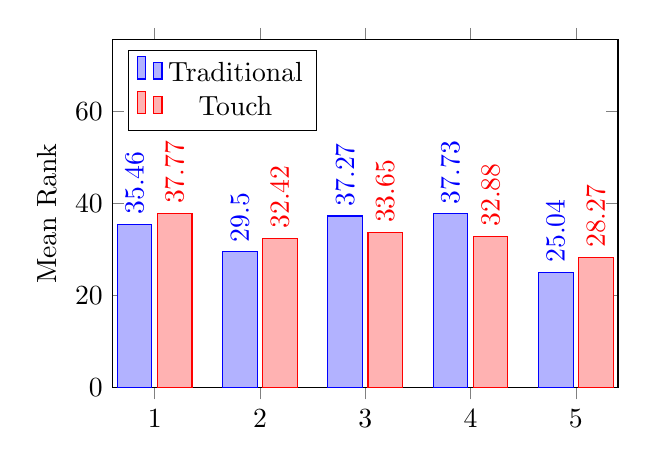
\begin{tikzpicture}
    \begin{axis}[
        ybar,
        every node near coord/.append style={rotate=90, anchor=west},
        ymin=0,
        width  = 8cm,
        height = 6cm,
        bar width=12.50pt,
        ylabel={Mean Rank},
        nodes near coords,
        xticklabel style={rotate=0},
        xtick = data,
        table/header=false,
        table/row sep=\\,
        xticklabels from table={
          1\\2\\3\\4\\5\\
          }{[index]0},
        enlarge y limits={value=1.00,upper},
        legend pos=north west
    ]
    \addplot table[x expr=\coordindex,y index=0]{35.46\\29.50\\37.27\\37.73\\25.04\\};
    \addplot table[x expr=\coordindex,y index=0]{37.77\\32.42\\33.65\\32.88\\28.27\\};
    \legend{Traditional, Touch}
    \end{axis}
\end{tikzpicture}
\caption{Kruskal-Wallis.}
\label{fig:Fig8}
\end{figure}

A small number of radiologists is used in the tests. Three of the five radiologists (1, 2 and 5) have shown that touch environment is better classified then traditional environment. Although, we must consider and understand the other two radiologist (3 and 4) results. This will be addressed in the discussion section. The Kruskal-Wallis test\footnote{
\textit{env}: environment (\textit{env}) with both traditional (\textit{tra}) and touch (\textit{tou}) options;

$\chi^2\textsubscript{env}$: Chi-Square of the environment (\textit{env});

$\alpha\textsubscript{env}$: Alpha value of the environment (\textit{env});
} revealed that radiologists have a significant main effect on touch environment ($\chi^2\textsubscript{tou} = 1.711$, $\alpha\textsubscript{tou} = 0.789$), against traditional environment ($\chi^2\textsubscript{tra} = 4.587$, $\alpha\textsubscript{tra} = 0.332$).


In the following sections (Figure \ref{fig:Fig8} - Figure \ref{fig:Fig12}) we describe the results in terms of the first and second order statistics, using the mean ($M\textsubscript{env}$) and standard deviation ($\sigma\textsubscript{env}$), as well as the standard error of the mean\footnote{
\textit{N}: the number of users (radiologists);

$sem\textsubscript{env}$: standard error of the mean for the environment (\textit{env});

$M\textsubscript{env}$: mean value of the environment \textit{env};

$\sigma\textsubscript{env}$: standard deviation of the environment \textit{env};
} that is defined as:

\begin{center}
$sem\textsubscript{env} = \sigma\textsubscript{env}/\sqrt{N}$
\end{center}

%where the statistically significant differences in the mean to substantive variables among all conditions, time performance, is improved on touch environment; hit rate score, although having less score for the touch environment, this condition show to be less important, since we conclude having enough annotation, even when those are not perfect. Also, preferences are statically significant different because radiologists are well known to be resistance to change work-flow.

\subsection{Performance}

Figure \ref{fig:Fig9} shows the mean time performance of the tasks as described in Section task. As above mentioned, for all the events, all coordinates of the annotation are saved and all the videos involving the user interaction are recorded.

\begin{figure}[h]  
\centering 

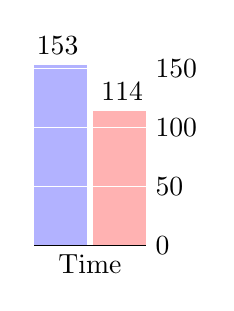
\begin{tikzpicture}
\begin{axis}[
    ybar, axis on top,
    height=4cm, width=3cm,
    bar width=0.75cm,
    ymajorgrids, tick align=inside,
    major grid style={draw=white},
    enlarge y limits={value=0.01,upper},
    ymin=0, ymax=160,
    axis x line*=bottom,
    axis y line*=right,
    y axis line style={opacity=0},
    tickwidth=0pt,
    enlarge x limits=true,
    legend style={
        at={(0.5,-0.2)},
        anchor=north,
        legend columns=-1,
        /tikz/every even column/.append style={column sep=0.5cm}
    },
    %ylabel={Seconds (s)},
    symbolic x coords={
       Time},
   xtick=data,
   nodes near coords={
    \pgfmathprintnumber[precision=0]{\pgfplotspointmeta}
   }
]
% TRADITIONAL
\addplot [draw=none, fill=blue!30] coordinates {
  (Time,153.40) };
% TOUCH
\addplot [draw=none,fill=red!30] coordinates {
  (Time,114.20) };

\end{axis}
\end{tikzpicture}% NO EMPTY LINE HERE!!!! 
\begin{tikzpicture}
\begin{axis}[
    ybar, axis on top,
    height=4cm, width=3cm,
    bar width=0.75cm,
    ymajorgrids, tick align=inside,
    major grid style={draw=white},
    enlarge y limits={value=0.01,upper},
    ymin=0, ymax=50,
    axis x line*=bottom,
    axis y line*=right,
    y axis line style={opacity=0},
    tickwidth=0pt,
    enlarge x limits=true,
    legend style={
        at={(0.5,-0.2)},
        anchor=north,
        legend columns=-1,
        /tikz/every even column/.append style={column sep=0.5cm}
    },
    %ylabel={Mean},
    symbolic x coords={
       NI},
   xtick=data,
   nodes near coords={
    \pgfmathprintnumber[precision=0]{\pgfplotspointmeta}
   }
]
% TRADITIONAL
\addplot [draw=none, fill=blue!30] coordinates {
  (Performance Time,39.20) };
% TOUCH
\addplot [draw=none,fill=red!30] coordinates {
  (Performance Time,40.00) };

\end{axis}
\end{tikzpicture}
\begin{tikzpicture}
\centering
\begin{axis}[
    ybar, axis on top,
    height=4cm, width=3cm,
    bar width=0.75cm,
    ymajorgrids, tick align=inside,
    major grid style={draw=white},
    enlarge y limits={value=0.01,upper},
    ymin=0, ymax=80,
    axis x line*=bottom,
    axis y line*=right,
    y axis line style={opacity=0},
    tickwidth=0pt,
    enlarge x limits=true,
    legend style={
        at={(0.5,-0.2)},
        anchor=north,
        legend columns=-1,
        /tikz/every even column/.append style={column sep=0.5cm}
    },
    %ylabel={Score},
    symbolic x coords={
       HRS},
   xtick=data,
   nodes near coords={
    \pgfmathprintnumber[precision=0]{\pgfplotspointmeta}
   }
]
% TRADITIONAL
\addplot [draw=none, fill=blue!30] coordinates {
  (Hit Rate,75.20) };
% TOUCH
\addplot [draw=none,fill=red!30] coordinates {
  (Hit Rate,50.60) };

\end{axis}
\end{tikzpicture}
\caption{Left: Time Performance Mean. Center: Number of Interactions (NI) Mean. Right: Hit Rate Score (HRS) Mean.} \label{fig:Fig9}
\end{figure}

\textit{Time}. On Figure \ref{fig:Fig9}: Left; we see that there is a significant main effect of the traditional input environment (M\textsubscript{tra}=153.4s, $\sigma$\textsubscript{tra}=40.88, {\mathop{\rm sem\textsubscript{tra}}}$\left({\bar x}\right)=18.28$) with radiologist maximum time spent of 210 seconds and radiologist minimum time spent of 109 seconds. For the touch input environment (M\textsubscript{tou}=114.20s, $\sigma$\textsubscript{tou}=51.71, {\mathop{\rm sem\textsubscript{tou}}}$\left({\bar x}\right)=23.12$) the radiologists take less time, however the standard error ({\mathop{\rm sem\textsubscript{tou}}}$\left({\bar x}\right)=23.12$) is higher on touch input environment. This result suggests that touch out-performs traditional environment in terms of time spent for doing the same tasks (Figure \ref{fig:Fig9}). This fact is aligned with previous work~\cite{forlines2007direct, watson2013deconstructing, kin2009determining}. On the previous bar-chart (Figure \ref{fig:Fig9}) we can better visualize the results.
  
\textit{Number of Interactions (NI)}.  From the Figure \ref{fig:Fig9}: Center; we can observe that there is a main effect on input of the total number of interactions (M\textsubscript{tra}=39.20, $\sigma$\textsubscript{tra}=4.65, {\mathop{\rm sem\textsubscript{tra}}}$\left({\bar x}\right)=2.08$), where the mean of the interactions on traditional (M\textsubscript{tra}=39.20) is less  (M\textsubscript{tou}=40) than the touch environment. Taking a deep look at the results, we can see that in the touch environment (M\textsubscript{tou}=40, $\sigma$\textsubscript{tou}=11.33, {\mathop{\rm sem\textsubscript{tou}}}$\left({\bar x}\right)=5.06$), has higher mean (M\textsubscript{tou}=40). This is desirable, since  we want to maximize the number of interactions and accuracy, minimizing the time speed. More interactions means that a higher number of annotations is obtained, thus a better input for the system is obtained in the same time. Thus, radiologists are engaging much more in the touch environments, as it can be seen on the previous bar-chart (Figure \ref{fig:Fig9}).

\textit{Hit Rate Score (HRS)}. In Figure \ref{fig:Fig9}: Right, it is shown the HRS, where the traditional environment (M\textsubscript{tra}=75.2, $\sigma$\textsubscript{tra}=22.72, {\mathop{\rm sem\textsubscript{tra}}}$\left({\bar x}\right)=10.16$) has a higher value then touch environment (M\textsubscript{tou}=50.6, $\sigma$\textsubscript{tou}=15.35, {\mathop{\rm sem\textsubscript{tou}}}$\left({\bar x}\right)=6.86$). One reason behind this results relies on the fact that the radiologists are less familiar with touch environments. Suggesting that higher rates
will be obtained if the spread use of the touch environments is accomplished. This will give room for improvements concerning  this type of environments.    


\subsection{User Experience}

Responses to the final questionnaire suggest that both interactions are adequate for analyzing medical images. Moreover no radiologist reported discomfort, dizziness or fatigue in neither environment.

\subsubsection{Motivational}

The motivational results are presented as \textit{Competence}, \textit{Autonomy}, \textit{Relatedness} and \textit{Immersion} (Figure \ref{fig:Fig10}) options.

\begin{figure}
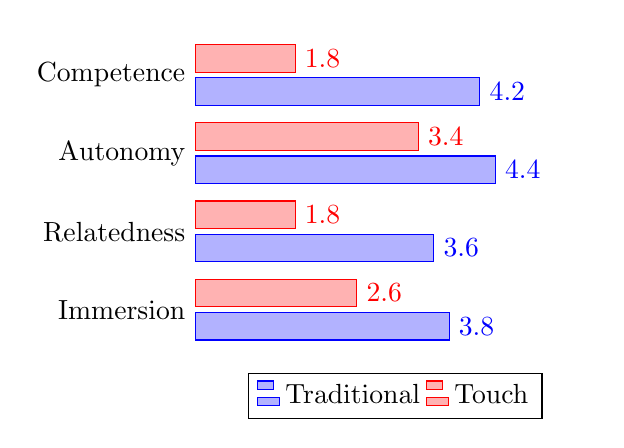
\begin{tikzpicture}
\begin{axis}[
align = center,
xbar,
y axis line style = { opacity = 0 },
axis x line       = none,
tickwidth         = 0pt,
height = 5.75cm,
enlarge y limits  = 0.20,
enlarge x limits  = 0.50,
symbolic y coords = {Immersion, Relatedness, Autonomy, Competence},
legend style={at={(0.5,-0.05)},
    anchor=north,legend columns=-1},
nodes near coords,
]
\addplot coordinates {
% TRADITIONAL
(3.8,Immersion)
(3.6,Relatedness)
(4.4,Autonomy)
(4.2,Competence)

};
\addplot coordinates {
% TOUCH
(2.6,Immersion)
(1.8,Relatedness)
(3.4,Autonomy)
(1.8,Competence)

};
\legend{Traditional, Touch}
\end{axis}
\end{tikzpicture}
\caption{Motivation Experience}
\label{fig:Fig10}
\end{figure}

\textit{Competence}. The experience of competence derives from challenge like personal effort of mastering challenges. The main outcome on traditional environment (M\textsubscript{tra}=4.2, $\sigma$\textsubscript{tra}=0.83, {\mathop{\rm sem\textsubscript{tra}}}$\left({\bar x}\right)=0.37$), showed that radiologists feel more comfortable in traditional environment, as it can be expected. On the other hand, for touch environment (M\textsubscript{tou}=3.4, $\sigma$\textsubscript{tou}=1.67, {\mathop{\rm sem\textsubscript{tou}}}$\left({\bar x}\right)=0.74$), radiologists showed a rated above average, however, lower than traditional environment. The maximum obtained value for touch is $\max_{}$(x\textsubscript{tou}) = 3 and for traditional is $\max_{}$(x\textsubscript{tra}) = 5.

\textit{Autonomy}. Experiencing greater autonomy will allow a person to feel more in control. The experience of autonomy derives from volition and willingness to perform a task. The traditional environment reflected (M\textsubscript{tra}=4.4, $\sigma$\textsubscript{tra}=0.89, {\mathop{\rm sem\textsubscript{tra}}}$\left({\bar x}\right)=0.4$) a high average level of autonomy with three radiologists choosing a $\max_{}$(x\textsubscript{tra}) = 5. For the touch environment we also have values above average (M\textsubscript{tou}=3.4, $\sigma$\textsubscript{tou}=1.14, {\mathop{\rm sem\textsubscript{tou}}}$\left({\bar x}\right)=0.5$), we also have a $\max_{}$(x\textsubscript{tou}) = 5 but just one radiologist scored this value.

\textit{Relatedness}. A heightened feeling of belonging to a group. Radiologists relatedness show us a touch environment below the average (M\textsubscript{tou}=1.8, $\sigma$\textsubscript{tou}=0.44, {\mathop{\rm sem\textsubscript{tou}}}$\left({\bar x}\right)=0.2$), where the $\max_{}$(x\textsubscript{tou}) = 2 and the $\min_{}$(x\textsubscript{tou}) = 1.  On the other hand, the traditional environment (M\textsubscript{tra}=3.6, $\sigma$\textsubscript{tra}=1.14, {\mathop{\rm sem\textsubscript{tra}}}$\left({\bar x}\right)=0.5$), we have the mean (M\textsubscript{tra}=3.6) above average, and the rest values typically normal. The $\max_{}$(x\textsubscript{tou}) = 5 and the $\min_{}$(x\textsubscript{tou}) = 2.

\textit{Immersion}. It is the sense that one is within the world. Immersion is supported by greater competence and autonomy. For motivational experience, the immersion values of traditional environment (M\textsubscript{tra}=3.8, $\sigma$\textsubscript{tra}=1.3, {\mathop{\rm sem\textsubscript{tra}}}$\left({\bar x}\right)=0.58$) are above average at the mean value (M\textsubscript{tra}=3.8). We have here a $\max_{}$(x\textsubscript{tra}) = 5 and the $\min_{}$(x\textsubscript{tra}) = 2, however two radiologists voted x\textsubscript{tra} = 5 the mean value (M\textsubscript{tra}=3.8) was not that high. The touch environment provided (M\textsubscript{tou}=2.6, $\sigma$\textsubscript{tou}=1.51, {\mathop{\rm sem\textsubscript{tou}}}$\left({\bar x}\right)=0.67$). Both, traditional and touch environments, have the standard deviation $\sigma$ \textgreater 1. This high standard deviation indicates that the data points are spread within a wider range of values on both environments.

\subsubsection{Pleasure and Enjoyment}

We present the results of \textit{Affect}, \textit{Enjoyment} and \textit{Intuitive Controls} (Figure \ref{fig:Fig11}).

\begin{figure}
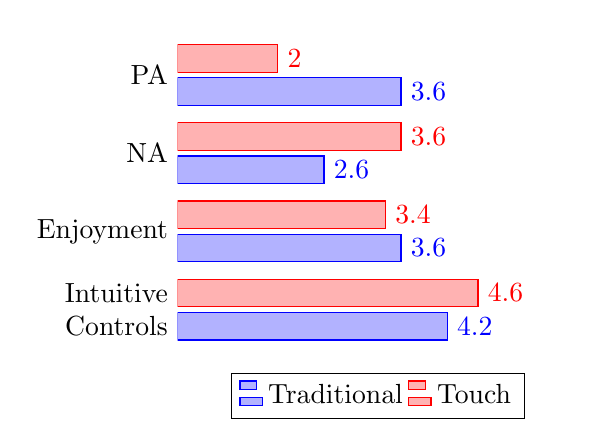
\begin{tikzpicture}
\begin{axis}[
align = center,
xbar,
y axis line style = { opacity = 0 },
axis x line       = none,
tickwidth         = 0pt,
height = 5.75cm,
enlarge y limits  = 0.20,
enlarge x limits  = 0.50,
symbolic y coords = {Intuitive\\Controls, Enjoyment, NA, PA},
legend style={at={(0.5,-0.05)},
    anchor=north,legend columns=-1},
nodes near coords,
]
\addplot coordinates {
% TRADITIONAL
(3.6,PA)
(2.6,NA)
(3.6,Enjoyment)
(4.2,Intuitive\\Controls)

};
\addplot coordinates {
% TOUCH
(2,PA)
(3.6,NA)
(3.4,Enjoyment)
(4.6,Intuitive\\Controls)

};
\legend{Traditional, Touch}
\end{axis}
\end{tikzpicture}
\caption{Overall Pleasure and Enjoyment of the Task}
\label{fig:Fig11}
\end{figure}

\textit{Affect}. The rise of the field of affective computing has placed an emphasis on understanding the affective and cognitive-affective responses that radiologists have to their technological interactions. Traditional environment is perceived as more positive (M\textsubscript{tra}=3.6, $\sigma$\textsubscript{tra}=0.54, {\mathop{\rm sem\textsubscript{tra}}}$\left({\bar x}\right)=0.24$), whereas the marginal negative affect for traditional environment (M\textsubscript{tra}=2.6, $\sigma$\textsubscript{tra}=0.54, {\mathop{\rm sem\textsubscript{tra}}}$\left({\bar x}\right)=0.24$) showed a typical correlation. The touch environment is perceived as more negative (M\textsubscript{tou}=2, $\sigma$\textsubscript{tou}=0.7, {\mathop{\rm sem\textsubscript{tou}}}$\left({\bar x}\right)=0.31$) then positive (M\textsubscript{tou}=3.6, $\sigma$\textsubscript{tou}=1.14, {\mathop{\rm sem\textsubscript{tou}}}$\left({\bar x}\right)=0.5$). As we can see, on the touch environment we do not have a typical correlation since the standard deviation and error for both positive ($\sigma$\textsubscript{tou}=0.7, {\mathop{\rm sem\textsubscript{tou}}}$\left({\bar x}\right)=0.31$) and negative ($\sigma$\textsubscript{tou}=1.14, {\mathop{\rm sem\textsubscript{tou}}}$\left({\bar x}\right)=0.5$) affect are not the same, as it occurs on traditional environment.

\textit{Enjoyment}. Intrinsic motivation is foundations of the enjoyment of interactive experiences, and can be attributed to volition and achievement inherent in the person. The traditional environment provides (M\textsubscript{tra}=3.6, $\sigma$\textsubscript{tra}=1.14, {\mathop{\rm sem\textsubscript{tra}}}$\left({\bar x}\right)=0.51$) which is almost the same as in the touch environment (M\textsubscript{tou}=3.4, $\sigma$\textsubscript{tou}=1.67, {\mathop{\rm sem\textsubscript{tou}}}$\left({\bar x}\right)=0.74$). This is a very interesting point in touch environments. It is known that although the radiologist exhibit more resistance in the use of touch, the enjoyment score high is competitive when comparing to traditional environments.
 
\textit{Intuitive Controls}. Controls are intuitive when they do not interfere with one's sense of presence being easily mastered. For the intuitive controls the overall system was high rated by radiologists, however the behavior of traditional environment (M\textsubscript{tra}=4.2, $\sigma$\textsubscript{tra}=0.44, {\mathop{\rm sem\textsubscript{tra}}}$\left({\bar x}\right)=0.2$) was less 8\% than touch environment (M\textsubscript{tou}=4.6, $\sigma$\textsubscript{tou}=0.54, {\mathop{\rm sem\textsubscript{tou}}}$\left({\bar x}\right)=0.24$).

\begin{figure}[h]  
\centering 

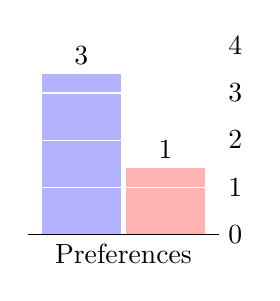
\begin{tikzpicture}
\centering
\begin{axis}[
ybar, axis on top,
height=4cm, width=4cm,
bar width=1cm,
ymajorgrids, tick align=inside,
major grid style={draw=white},
enlarge y limits={value=0.01,upper},
ymin=0, ymax=4,
axis x line*=bottom,
axis y line*=right,
y axis line style={opacity=0},
tickwidth=0pt,
enlarge x limits=true,
legend style={
    at={(0.5,-0.2)},
    anchor=north,
    legend columns=-1,
    /tikz/every even column/.append style={column sep=0.5cm}
},
symbolic x coords={
   Preferences},
xtick=data,
nodes near coords={
\pgfmathprintnumber[precision=0]{\pgfplotspointmeta}
}
]
% TRADITIONAL
\addplot [draw=none, fill=blue!30] coordinates {
(Preferences,3.4) };
% TOUCH
\addplot [draw=none,fill=red!30] coordinates {
(Preferences,1.4) };

\end{axis}
\end{tikzpicture}% NO EMPTY LINE HERE!!!! 
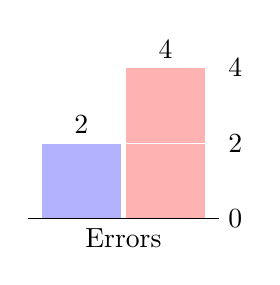
\begin{tikzpicture}
\centering
\begin{axis}[
ybar, axis on top,
height=4cm, width=4cm,
bar width=1cm,
ymajorgrids, tick align=inside,
major grid style={draw=white},
enlarge y limits={value=0.01,upper},
ymin=0, ymax=5,
axis x line*=bottom,
axis y line*=right,
y axis line style={opacity=0},
tickwidth=0pt,
enlarge x limits=true,
legend style={
    at={(0.5,-0.2)},
    anchor=north,
    legend columns=-1,
    /tikz/every even column/.append style={column sep=0.5cm}
},
symbolic x coords={
   Errors},
xtick=data,
nodes near coords={
\pgfmathprintnumber[precision=0]{\pgfplotspointmeta}
}
]
% TRADITIONAL
\addplot [draw=none, fill=blue!30] coordinates {
(Errors,2) };
% TOUCH
\addplot [draw=none,fill=red!30] coordinates {
(Errors,4) };

\end{axis}
\end{tikzpicture}
\caption{Left: Preferences Mean. Right: Number of Errors Mean.} \label{fig:Fig12}
\end{figure}

\subsection{Preferences}

We asked radiologists to rank (Figure \ref{fig:Fig12}) the environments in order of preferences (scale 1-4, 1=worst and 4=best). The quiz revealed that radiologists ranked the environments differently. Pairwise, some comparisons revealed that traditional environment (M\textsubscript{tra}=3.4, $\sigma$\textsubscript{tra}=0.55, {\mathop{\rm sem\textsubscript{tra}}}$\left({\bar x}\right)=0.24$) is ranked higher than touch environment (M\textsubscript{tou}=1.4, $\sigma$\textsubscript{tou}=0.55, {\mathop{\rm sem\textsubscript{tou}}}$\left({\bar x}\right)=0.24$). Taking a deep observation, we can see that even when the means are different, we have the same standard deviation and error ($\sigma$\textsubscript{}=0.55, {\mathop{\rm sem\textsubscript{}}}$\left({\bar x}\right)=0.24$) what could mean the same behavior and decisions. The $\max_{}$(x\textsubscript{tra}) = 4 and $\min_{}$(x\textsubscript{tra}) = 3. Regarding the touch environment we obtain a $\max_{}$(x\textsubscript{tou}) = 2 and a $\min_{}$(x\textsubscript{tou}) = 1. Two radiologists voted x\textsubscript{tra} = 4 and three radiologists voted x\textsubscript{tra} = 3. And two radiologists voted x\textsubscript{tra} = 2 and three radiologists voted x\textsubscript{tra} = 1. These questions showed us that the touch environment has a radiologists resistance to change environment and to prefer the touch environment.

\subsection{Errors}

Another number, the error counter (Figure \ref{fig:Fig12}), may have been regardless, so the method chosen error counter did not affect the conclusion about overall measures from performance and the total number of iterations process. The errors (Figure \ref{fig:Fig12}) must take in consideration when trying to understand accuracy and time spending on annotations repeat.

On our study we evaluated the error as each time a radiologist press the \textbf{Clear drawing} button and repeat the annotation again. For that task we had one radiologist doing two errors on the traditional environment. And for the touch environment we had two radiologists doing two errors each.

\section{Discussion}

There are no direct effects between the motivational experience, pleasure and enjoyment experience results on any of the experience measures. The only interaction involving both environments suggests that each environment has its own pros-and-cons. This make sense as the radiologists would be more fatigued from having different environments, where the second environment usual supported a more fatigued radiologist then the first environment for trivial reasons.

The differences resulting from environment type showed that even traditional environment out-performed touch environment in terms of motivational results like competence, autonomy, relatedness and immersion. And even when traditional environment still out-performed pleasure and enjoyment results like positive affect, enjoyment and intuitive controls, we still have touch environment improvements on time performance and number of interactions. These results suggest that there is a speed/accuracy improvement on the trade-off as a result of using touch environment, and that radiologists engaged more with the system in the touch environment.

Furthermore, this results show that radiologists are significantly happier (positive affect) remaining on their usual work-flow environment, the traditional environment, having more joy of interaction (enjoyment) when using those. In addition, radiologists have higher competence, autonomy, relatedness and immersed, with a mental involvement on the tasks, by the use of traditional environment. Also, the hit rate scored a remaining feeling with the traditional environment even when the touch environment has a less 24 score points then traditional environment.

Finally radiologists rank traditional environment higher than touch environment. The differences between traditional and touch environments for performance, can not be related to differences in intuitive controls, as we found no main effects on less traditional ratings of intuitive controls. The general assumptions contrast with the touch environment as it is more intuitive, but on the same time, more fatiguing. Also, radiologists resistance of health-care information technology~\cite{bloom1988structure} (HIT) usage by integrating the technology acceptance and resistance to change the work-flow is a well known issue and represents the rank preferences on this study.

The radiologists systematically rate their motivational, pleasure and enjoyment experience with traditional environment better than touch environment. This happens for several reasons. First, a new environment (as the touch one), constitutes a higher challenge for radiologists, since it is not the typical work-flow of interaction. Second, the radiologists actually performed better in terms of time performance and more number of interactions with the touch environment than the traditional. The higher number of interactions also suggests that radiologists are engaging more with the touch environment. Fourth, we observed that there
is an attraction the  nature~\cite{kin2009determining} of touch environment interactions in medical image diagnosis context~\cite{seibel2005medical}.

Although, radiologists provided higher score accuracy (Figure \ref{fig:Fig9}: Right) at Hit Rate Score (HRS) with traditional environment over touch, this will not be an important issue, since we did not obtain any zero (HRS = 0) annotations. Furthermore, a nearly perfect annotation accuracy of HRS = 3 is not as important as its corresponding time. This happens, since the radiologists are interested just on the approximated region of interest disregarding its accuracy. This means that the time spent becomes the most important aspect to take into account. Thus, the touch environments becomes the most relevant environment, since the running time figures are superior when compared with traditional environments.

Combined with a higher number of interactions, the time performance of touch environment suggests that in less time, the radiologists perform more annotations. This brings us to a new conclusion that touch is more informative, in sense that more annotations are provided. This suggests that traditional environment is less efficient. However, the global experience results tend to remain at the traditional environment suggesting the medical resistance of change

In conclusion, although the radiologists are famously known to be resistant to changes in their work-flow, it is interesting to note the scores obtained
for enjoyment and intuitive which at the same level or higher when compared to traditional environments. Also, we should highlight that the number of annotations is also higher in touch environment. This suggests that the use of touch in medical work-flow is still in its infancy and as such, there is an open door for reaching further improvements in touch based interfaces. 

\section{Conclusion}

In this work, we propose and evaluate a set of results to a medical image diagnosis user interface on traditional and touch environments. Our analysis describes performance and experience on both environments using a simple user interface and several validated scales. We fully describe our proposed interaction design techniques and detail the aspects of our user interface interaction.

We make several contributions on this study. First, we show that touch environment improved on performance metrics of time and also number of interactions. Second, we show that despite this improvement came at an experience cost, by the variety of measures related to motivational, pleasure and enjoyment experience. Third, we demonstrate an efficient and effective method for gathering performance and experience with medical image diagnosis user interfaces. At the end, we discuss the implications of improved performance by the trade-off of experience on touch environment for medical image diagnosis.

There are still several issues to work in a nearly future. From the medical resistance to the finger cover areas. Also, this method for understanding performance and experience could also be extended radiology DICOM image like breast screening cancer diagnosis, since this problem is aligned to the one described herein.

Our research is applied to a novel domain: the medical image diagnosis; where touch user interface produces a superior time performance regarding  the traditional use. Also, it has more intuitive control and a higher number of interactions, giving a more information concerning the annotation of the lesions in shorter time.

\section{Acknowledgments}

I would like to convey our gratefulness to Hospital Fernando Fonseca (HFF) for the collaboration. I would specially like to thank the Doctors Clara Aleluia, Gisela Andrade, William Schuitt and Ana Sofia Germano from the HFF for the generous support and medical expertise. My appreciation goes also to Bruno Cardoso and Bruno Dias for help and above all for the good companionship. Thanks to Professors Daniel Sim\~{o}es Lopes and Daniel Mendes for the support. Last but not least, thank to Joana Teixeira and L\'{i}dia Freitas for the feedback. This work was partially supported by Funda\c{c}\~{a}o para a Ci\^{e}ncia e a Tecnologia (FCT) and Instituto Superior T\'{e}cnico (IST) through the RD0461-LARSys-ISR-CC930403:UID/EEA/50009/2013 project, BL89/2017-IST-ID grant.

% Balancing columns in a ref list is a bit of a pain because you
% either use a hack like flushend or balance, or manually insert
% a column break.  http://www.tex.ac.uk/cgi-bin/texfaq2html?label=balance
% multicols doesn't work because we're already in two-column mode,
% and flushend isn't awesome, so I choose balance.  See this
% for more info: http://cs.brown.edu/system/software/latex/doc/balance.pdf
%
% Note that in a perfect world balance wants to be in the first
% column of the last page.
%
% If balance doesn't work for you, you can remove that and
% hard-code a column break into the bbl file right before you
% submit:
%
% http://stackoverflow.com/questions/2149854/how-to-manually-equalize-columns-
% in-an-ieee-paper-if-using-bibtex
%
% Or, just remove \balance and give up on balancing the last page.
%
\balance

\bibliographystyle{acm-sigchi}
\bibliography{sample}
\end{document}
